\documentclass[conference]{IEEEtran}
\IEEEoverridecommandlockouts
% The preceding line is only needed to identify funding in the first footnote. If that is unneeded, please comment it out.
\usepackage{cite}
\usepackage{amsmath,amssymb,amsfonts}
\usepackage{algorithmic}
\usepackage{graphicx}
\usepackage{textcomp}
\usepackage{xcolor}
\def\BibTeX{{\rm B\kern-.05em{\sc i\kern-.025em b}\kern-.08em
    T\kern-.1667em\lower.7ex\hbox{E}\kern-.125emX}}
\begin{document}

\title{Systems of Digital Twins and Physical Systems: Interoperability, Decentralization, and Mobility in Robotic Applications}

\author{\IEEEauthorblockN{Felix Girke}
\IEEEauthorblockA{\textit{Dept. of Comp. Science \& Engineering} \\
\textit{Frankfurt University of Applied Sciences}\\
Frankfurt a.M., Germany \\
https://orcid.org/0009-0004-3967-6750}
\and
\IEEEauthorblockN{René Harmann}
\IEEEauthorblockA{\textit{Dept. of Comp. Science \& Engineering} \\
\textit{Frankfurt University of Applied Sciences}\\
Frankfurt a.M., Germany \\
rene.harmann@fb2.fra-uas.de}
\and
\IEEEauthorblockN{Eric Guiffo Kaigom}
\IEEEauthorblockA{\textit{Dept. of Comp. Science \& Engineering} \\
\textit{Frankfurt University of Applied Sciences}\\
Frankfurt a.M., Germany \\
kaigom@fb2.fra-uas.de}
}

\maketitle

\begin{abstract}
Whereas digital twins are receiving an increasing
attention, their implementation has been predominated by mono-
lithic and static solutions. A resulting issue is the lack of a
modular integration and seamless interplay of digital twins when
it comes to adapt and support varying industrial and societal
applications. Another drawback arises from limited services that
digital twins can provide as the physical system is extended
with new components and/or separated from constituting parts,
giving rise to a metamorphosic system of systems. Furthermore,
the respective mobility of physical systems and citizens assumed
to interact with them via their digital surrogates is hardly
transformed into industrial and societal opportunities, such as
a pervasive and itinerant human-robot-interaction ($\pi$-HRC).
Within the scope of our Metarobotics framework that propels
$\pi$-HRC, we address these challenges by leveraging on the OPC
UA standard to develop portable data connectors that move
with and give access to the data source, which is the associated
physical system. Our Raspberry-Pi driven connector encapsulates
a digital twin of the corresponding system and its offered services
to capture the loose coupling and decentralization of systems
and systems even remotely and in motion. Each data connector
semantically interoperates with any OPC UA capable system
and device via wireless communication. This opens up new
opportunities for different monitoring (and control) modalities
of large scale systems whose physical or/and virtual constituting
subsystems are distributed across distinct geographical locations
in the industrial and societal realm. We apply our framework
to a mobile multi-arm robotic system with edge-computing
capabilities and demonstrate the performance of its monitoring
functionality from the cabin of a moving train in city traffics
in practice. We provide experimental measurements results and
highlight the usefulness and effectiveness of our approach.
% To solve the problem of different interfaces for different robots a data connector is developed.
% It creates a interoperable, decentralized network for a robot system using the Open Platform Communication Unified Architecture (OPC-UA) standard.
% Using this network a flexible digital twin is created in Isaac Sim to visualize the data of the robot system.
% To monitor the robot system from everywhere the possibility of an remote access to the data connectors is set up.
\end{abstract}

\begin{IEEEkeywords}
Robotics, Digital Twins, System of Systems, Industry 4.0, Industry 5.0, Society 5.0, Human-Robot-Interaction
% OPC-UA, interoperable, decentralized, digital Twin, Isaac Sim, remote access
\end{IEEEkeywords}

\section{Introduction}
Every robot manufacturer develops their own way of communication with their robots.
This leads to problems when trying to build a robot system with multiple robots from different brands.
In this example two robot arms from Kinova are to be mounted on a Husky mobile robot platform from Clearpath.
The Husky uses Robot Operating System (ROS) to communicate internally while the robot arms use the Kortex API from Kinova.
To combine them into one digital twin they should be on one standard.
For this a data connector is developed on the Open Platform Communication Unified Architecture (OPC-UA) standard.
Its purpose is to act as a layer between the robot specific language and the outside world, in this example the digital twin.
To add flexibility the robot data isn't collected on one central server but every robot has its own server.
Because of this decentralized approach every client can choose to connect only to the servers it needs to.
For example if only one of the robot arms is mounted on the Husky the digital twin can connect to only this one robot arm while the other robot arm can be used otherwise.
\section{State of the art}
The Task of connecting different robots together to form a network has been attempted by different Teams.
In \cite{SotaCAN} three robotic arms have been connected using CAN for a cooperative Task.
The translation between the robots and the local CAN network is achieved by using a microcontroller on every robot.\\
A similar Network was build in \cite{SotaROS} but here ROS is used as an communication protocol.
Unlike in the first paper the robots aren't the same but they all have native support for ROS so there is no need for a translation layer between the robot an the network.\\
To create more flexibility in such a network in \cite{StoaROStoOPCUA} a Interoperability between ROS and a OPC-UA is achieved by integrating them into a local cloud framework.\\
A completely different approach was made in \cite{SotaRaconteur} and \cite{SotaFusion}.
Here a middleware was developed to make a network for the different heterogeneous robots.
While the Robot Raconteur software from \cite{SotaRaconteur} is open source, the CorteX software from \cite{SotaFusion} is not.
Furthermore CorteX is build specifically for a robot system working in a Fusion Reactor while Robot Raconteur is build to be an ecosystem for different robots.
% -- Robot Raconteur Middleware for robots (https://ieeexplore.ieee.org/abstract/document/10260569)\\
% -- CorteX, plug and play, distributed system of systems, Fusions Reactor, ähnlich OPC UA aber mit control (https://www.mdpi.com/2218-6581/10/3/108)\\
% -- Interoperability ROS und OPC-UA (https://ieeexplore.ieee.org/abstract/document/9816962)\\
% -- Can Bus, 3 Arme, dezentral, mikocontroller, lokal (https://link.springer.com/chapter/10.1007/978-981-15-5281-6\_30)\\

% --heterogen Robot network, all using ros (https://ieeexplore.ieee.org/abstract/document/9707460)\\
% homogen Robot network peer to peer, find path (https://ieeexplore.ieee.org/document/9196672)\\
\section{Advantages of OPC-UA}
The fourth industrial revolution is about making machines and products "smart" to make decisions and control the manufacturing process on their own \cite{Industry4}.
To make these decisions they need to be connected to other machines and resources to get data on which the decisions are based.
On this need for connection many different standards where build.
Two of the most common are Message Queuing Telemetry Transport (MQTT) and OPC-UA \cite{CommTechnology}.
Both are build on the Transmission Control Protocol (TCP).
UA is a standard published by the Open Platform Communication Foundation in 2008 and is an "platform independent service-oriented architecture that integrates all the functionality of the individual OPC Classic specifications into one extensible framework" \cite{OPCUA}.
While MQTT is only event driven OPC-UA is both a Remote Procedure Call (RPC) and an PubSub mode \cite{OPCUA}. 
OPC-UA is not as lightweight as MQTT but the information model is much more semantic and it is much Therefore performant than MQTT \cite{CommunicationCommarison}.
In 2014 the Fraunhofer IOSB has started the open62541 library for C in cooperation with RW-TH Aachen and the TU Dresden \cite{open62541}.
Today this is one of the feature richest open source implementation of the OPC-UA standard \cite{ComparOPCUAPaper}.
On the other hand there is FreeOpcUa as an very easy to use python library.
Its performance might not be as good as the C-library but with a powerful PC it isn't the limiting factor and can also be used.\\
The architecture of OPC-UA with an standard between all servers and clients makes it perfect for building a decentralized and interoperable network.
It is easy to have multiple servers and clients in one network and every client can talk to every server simultaneously.
This makes the network very flexible.\\

Another feature of OPC-UA is the support for multiple security critical functionalities like session encryption, message signing and authentication. \cite{OPCUA}
\section{Development of the data connector}
Depending on the robot it might be possible to install software on it.
If this is the case there is no need for additional Hardware.
The Husky PC runs ROS, so it is possible to create an ROS package with an OPC-UA Server.
The Kinova robotic arms on the other Hand it is not possible to install software, so a Raspberry Pi is used as a data connector which gets the data from the robot and makes it accessible via an OPC-UA server.\\
As Hardware for the stand-alone device a Raspberry PI 3B+ is used due to it's very versatile nature. It can connect to robots via Ethernet, USB or various GPIO pins.
Furthermore it is powerful enough to handle an OPC-UA server and communicate to a robot at the same time.
Because of its size it can be mounted directly on the Kinova robot without interfering the movement of the robot (Fig. \ref{fig:dataConectorPic}).
\begin{figure}[htbp]
    \centerline{\includegraphics[height=4.5cm]{Pictures/PiGehaeuseVorne.jpeg}\hspace{0.1cm}\includegraphics[height=4.5cm]{Pictures/PiAmKinova.jpeg}}
    \caption{The data connector mounted directly on the Kinova robot}
    \label{fig:dataConectorPic}
\end{figure}
The data connector can even be powered by the USB ports of the Kinova robot, so no additional power source is needed.\\
The Code is split into three main parts (Fig. \ref{fig:dataConectorStructure}).
\begin{figure}[htbp]
    \centerline{\includegraphics{Pictures/dataConectorStructure.pdf}}
    \caption{Code structure of the data connector}
    \label{fig:dataConectorStructure}
\end{figure}
One part is the communication to the robot via the Kortex API, the second part is the OPC-UA server with the open62541 library.
The connection to the robot is done on the UDP protocol and the data is requested via the cyclic feedback function of the Kortex API, because it is the fastest way to get the data from the robot.
The main code part in the middle  starts a thread for the connection to the robot and a thread for the OPC-UA server.
It also connects the data from from the robot class to the OPC-UA server class.
To do this, there is a map defined that connects the function needed to get the data from to robot to the name of the variable on the OPC-UA server.
Therefore it is very easy to add or remove variables from the OPC-UA Sever by adding or removing an entry from this map.\\
This system allows a lot of flexibility. The data connector is plug and play capable with any of the Kinova robot arms because they are all using the Kortex API.
If the connector is to be used with another robot from another manufacturer, it is enough to just write a new connection to the robot and modify the main code.
It is also possible to prepare the connection protocol for multiple robots from different manufacturers and let the main code detect which robot is connected and which protocol is to be used.

\section{Performance Tests}
To ensure the data doesn't take to long from the robot to a client a series of performance tests are conducted.
These can be split into two parts. 
First getting the data from the robot to the data connector and second get the data from the data connector to the client.
Every test is made with 5 samples. Every sample is the average speed of the first 1000 data requests.
\subsection{Getting data from the robot}
The Raspberry Pi 3B+ is directly connected to the Kinova robot via an ethernet cable.
With UDP as communication standard the Raspberry Pi can get the up to 1400 datasets per second from the Kinova robot (Fig. \ref{fig:KortexAPISpeed}).
That is even more than the 1000 datasets per second, that Kinova claims \cite{KortexUDP}.\\

\begin{figure}[htbp]
    \centerline{\includegraphics[width=8cm]{Pictures/KortexAPISpeed.pdf}}
    \caption{Frequency with which the Raspberry Pi 3B+ can get data from the Kinova arm}
    \label{fig:KortexAPISpeed}
\end{figure}
A dataset consists of all the data the robot has to offer, which are over 50 data points.
If the OPC-UA server is running parallel on the Raspberry Pi the frequency is lower, around 1kHz.
If one client is simultaneously requesting data from the OPC-UA server the frequency isn't really affected, but if there are more clients the frequency begins to drop.
\subsection{Getting Data from the data connector}
To get the data from the data connector two different PCs are used. One midrange Laptop (Intel 11.Gen Core i7-1165G7, Realtek Semiconductor
RTL8152 Fast Ethernet Adapter) and an high end Tower PC (Intel 13.Gen Core i9-13900KF, Realtek Gaming R2.5GbE Family Controller).
The PCs and the data connector are all connected to the same Router (tp-link Archer C80 AC1900 MU-MiMO).\\

\begin{figure}[htbp]
    \centerline{\includegraphics[width=8cm]{Pictures/OPCUASpeed1D.pdf}}
    \caption{Frequency with which data can be requested from the OPC-UA server}
    \label{fig:OPCUASpeed1D}
\end{figure}
In Fig. \ref{fig:OPCUASpeed1D} different libraries are used for the client to request one value from the data connector.
On the Laptop the C-library open62541 is faster than the python library FreeOpcUa.
On the Tower PC the python library is even faster than the C-library on the Laptop.
If these results are compared to the ping between these PCs and the data connector (Fig. \ref{fig:PingDiagram}) it can be concluded that the python library on the Tower PC is running close to the actual limit of the network.\\

\begin{figure}[htbp]
    \centerline{\includegraphics[width=8cm]{Pictures/PingDiagram.pdf}}
    \caption{Ping to the data connector}
    \label{fig:PingDiagram}
\end{figure}
If multiple clients are started in parallel on the Tower PC there is a slight decrease in the frequency with which the data can be requested from the data connector (Fig. \ref{fig:OPCUASpeed1D}).\\
\begin{figure}[htbp]
    \centerline{\includegraphics[width=8cm]{Pictures/OPCUAMultipleDatenAufEinmal.pdf}}
    \caption{Frequency with which different datasets can be requested from the OPC-UA server}
    \label{fig:OPCUAMultipleDatenAufEinmal}
\end{figure}
In the last attempt (Fig. \ref{fig:OPCUAMultipleDatenAufEinmal}) datasets with different amounts of values are requested from the data connector via the Tower PC using the python library.
The difference between 1 value an 10 values in one request is relative small (18 packages), between 10 and 20 values this gap widens (47 packages) and between 20 and 30 it is even bigger (64 packages).
It is clearly not a linear decrease but also not an exponential one. 
Both the PC and the Raspberry Pi are consuming less than 20\% of the CPU so this isn't the bottleneck.
The size of the package gets bigger with every additional value and there seems to be no limit at which the packages are split.
If all 57 values are requested in one package its size is 2538 bytes.
This length is depending mostly of the name of the values because the longer they are, the bigger the package.\\
The best way to request this many values is in two packages with 28 and 29 values each.
The frequency is half that of one 30 value package but this is still nearly two times as fast as requesting all 57 values in one package.
\section{Husky battery Soc}
Not all data can just be displayed on the OPC-UA server.
For Example the State of Charge (SoC) of the Husky is only visible on a four segment display and not available as a discrete value.
The display is probably tuned for an lithium ion battery so it is very inaccurate for the sealed lead-acid battery that is currently powering the Husky.
Because of this one sided tuning it shows only around 50\% SoC with an full battery and after a short time of usage it shows 0\% SoC.
To create a better estimation of the SoC a ROS package is created that uses the measured current and potential of the battery and publishes an estimation of the SoC tuned for the used SLA battery.
This data is also published on the OPC-UA server.
\subsection{Estimating the SoC}
In the documentation of the Husky Fig. \ref{fig:EndladekuvenSLA} can be found.
\begin{figure}[htbp]
    \centerline{\includegraphics[width=8cm]{Pictures/EndladekuvenSLA.png}}
    \caption{Discharge time over different currents for the SLA battery of the Husky \cite[p.21]{SLAKurven}}
    \label{fig:EndladekuvenSLA}
\end{figure}
With this curves the SoC can be estimated using the measured current and potential of the battery.
First the functions of the curves have to be approximated. For this a 4th degree polynomial is used.
It represents the curves fairly accurate within the usable range of the battery.
To make the estimation easier the x and y data is flipped before approximation.
The results are functions for different currents that can be used to estimate the time of possible usage.
Comparing this value with the maximum time the battery can be used produces the percentage of the battery that is already consumed.
\subsection{Validating the SoC estimation}
To validate the estimation the battery is performs a complete discharge cycle and the estimated SoC, the current and the potential of the battery are recorded.
In Fig. \ref{fig:SoCUeberZeit} is the estimation of the SoC over one discharge cycle shown.\\

\begin{figure}[htbp]
    \centerline{\includegraphics[width=8cm]{Pictures/SoCUeberZeit.pdf}}
    \caption{Comparison between the theoretical SoC and the estimated SoC over one discharge cycle}
    \label{fig:SoCUeberZeit}
\end{figure}
As a comparison there is also the theoretical SoC calculated from the average current shown.
First of all it is visible that the battery don't start at 100\% it is likely that the battery don't hold a full charge anymore because of wear.
The estimated SoC is an moving average over 100 values but still there is some noise in the data.
Thats because the measured potential and current are very noisy (Fig. \ref{fig:SpannungStromUeberZeit}).
\begin{figure}[htbp]
    \centerline{\includegraphics[width=4cm]{Pictures/SpannungUeberZeit.pdf}\includegraphics[width=4cm]{Pictures/StormUeberZeit.pdf}}
    \caption{Measured potential and current over one discharge cycle of the Husky battery}
    \label{fig:SpannungStromUeberZeit}
\end{figure}
There are also big spikes in the data around 150, 210 and 480 minutes.
At the same time there are spikes in the current but not in the potential.
For this reason it is likely that this is due to poor measurements.
At 270 minutes there is also a big spike in the current but because there is also a spike in the potential of the battery, the the SoC hardly changes.
Because there is no documentation on which sensor Clearpath is using or how the measurements are made it can't be replicated.
But the the new SoC estimation is much more precise than the old one and an underestimation of the SoC leads to an bigger safety margin which is also useful.
\section{Digital twin}
The digital twin is build in Isaac Sim.
This is a simulation tool for robots and part of the NVIDIA Omniverse.
Isaac Sim works with usd files but there are native tools to convert other file types like urdf to usd so most robots can be easily imported.\\
In order to be able to connect to the OPC-UA server, a client is needed.
The best way to implement this is via an extension for Isaac Sim.
To reflect the modularity of the robot system and the decentralized network approach, multiple different configurations of the robot system are created.
The extension has an Graphical User Interface (GUI) in which the configuration of the robot system can be chosen.
Independent form the chosen configuration it is also possible to choose to which OPC-UA server you want to connect.
This allows to test a robot configuration you don't have. 
For example it could be tested if the Husky will tip over when the Kinova arm performs a specific movement, even if you don't have a Husky robot.
Just load a configuration with the Husky and a Kinova arm and connect to it.
The Kinova arm can now be moved with the controller and you can test any movement.\\
Furthermore it is possible to open a graph in which any data from the robot can be displayed.
So the non-visible data like current or temperature can be visualized.
Even if you don't use one of the robots in the robot system it is still possible to connect to the robot to keep an eye on its vitals.\\
To make the digital twin more realistic you can choose in the GUI to load a 3D scan of the university as an environment for the digital twin (Fig. \ref{fig:CompareDigitalReal}).
\begin{figure}[htbp]
    \centerline{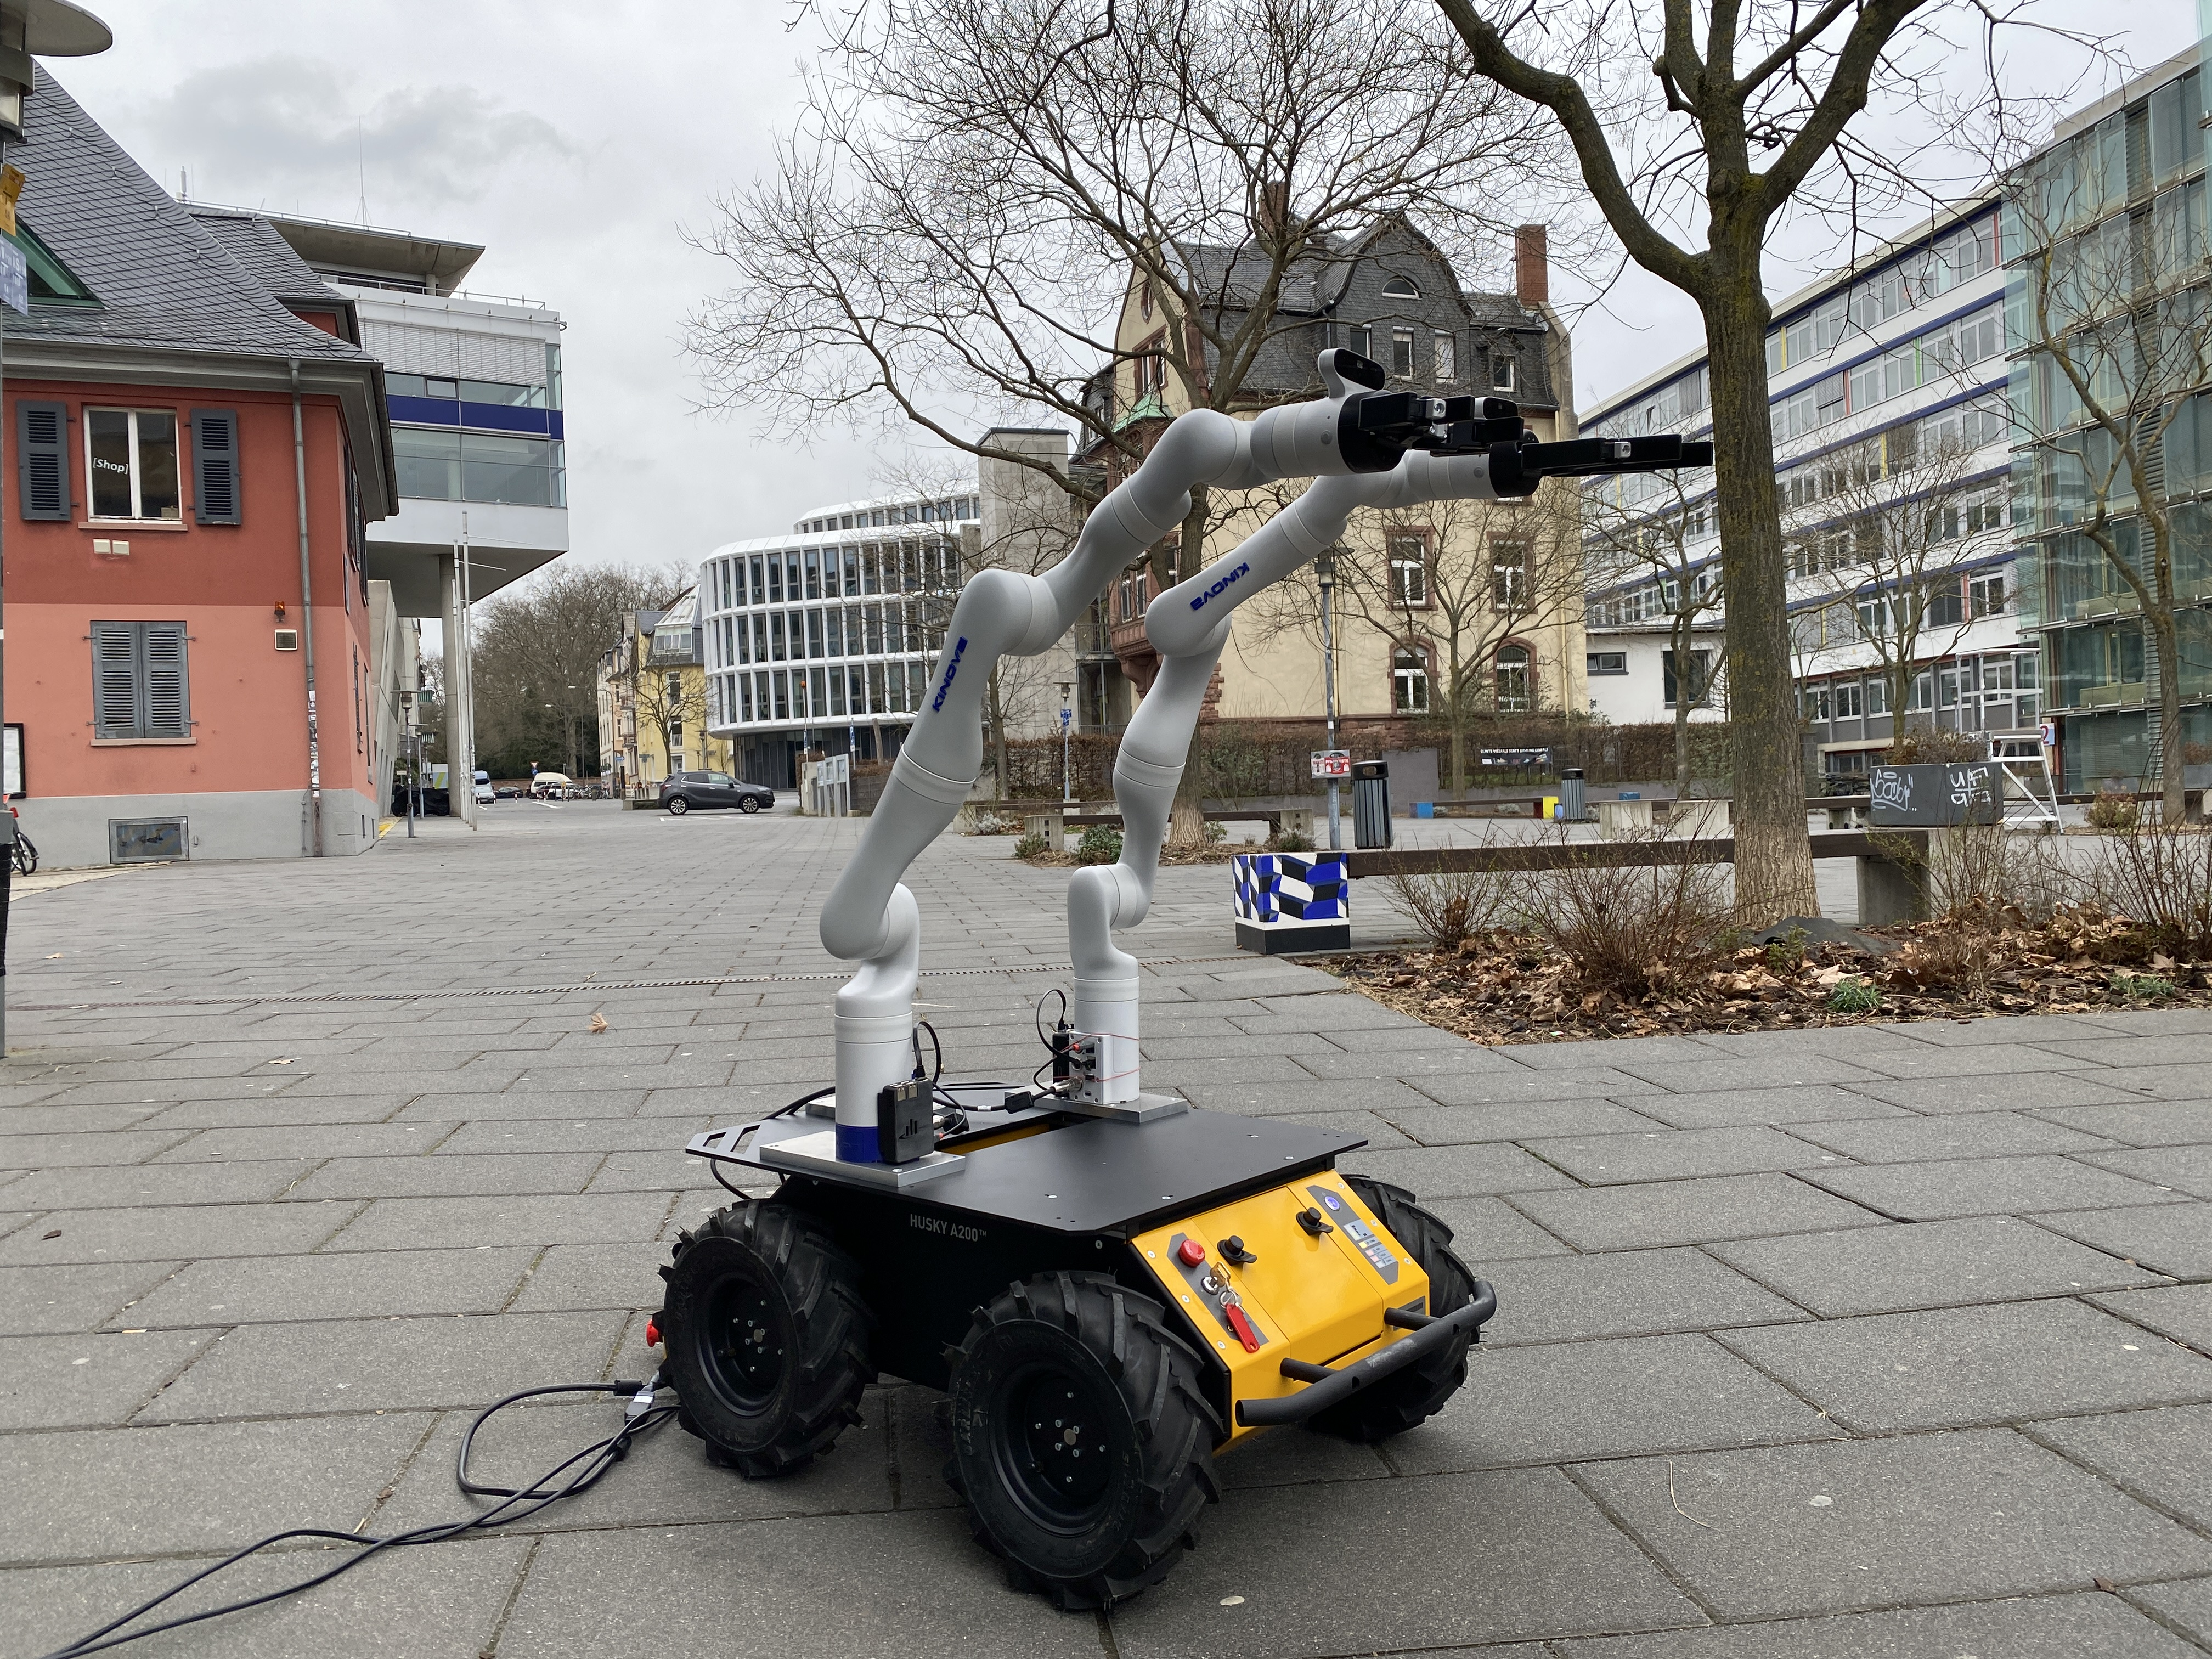
\includegraphics[width=4cm]{Pictures/DigitalerTwinNachgestellt1.JPG}\includegraphics[width=4cm]{Pictures/DigitalerTwinNachgestellt2.png}}
    \caption{Comparison of the digital twin (left) and the real robot (right)}
    \label{fig:CompareDigitalReal}
\end{figure}

\section{Remote access}
To monitor the robot system from everywhere a remote access to the data connectors is needed.
For this an mobile 5G router is mounted on the Husky. To this Router all the data connectors are connected.
On the router an VPN is installed, so to connect to a data connector a client has to connect to the router via the VPN first.
Afterwards the connection to the data connector is identical as before.
In Fig. \ref{fig:RemoteAccess} an example is shown where the client is accessing the battery data of the Husky from a train while the Husky is in the lab of the university.
\begin{figure}[htbp]
    \centerline{\includegraphics[width=8cm]{Pictures/ZugZugriff.png}}
    \caption{Example of the remote access to the data connector of the robot in the university lab from a Train}
    \label{fig:RemoteAccess}
\end{figure}
To achieve this a special Sim Card for the router is needed.
It has to have an public IP-Address. For Sim Cards this is not common.
Normally they get their Messages like push notification via a Google or Apple server.
Without an public IP-Address it is not possible to reach the VPN server.
Alternately a software like ngrok can be used to to make a tunnel to the data connector. Therefore no public IP-Address is needed but for every data connector a separate tunnel is required.
\section{Discussion}
\section{Conclusion}
It could be shown in this paper that it is possible to create an decentralized and interoperable network using the OPC-UA standard.
Furthermore with the data connector the whole setup is very flexible and can be added to every Kinova robot arm using the Kortex API.
It is also possible to expand the data connector to work with many different robots from different manufactures.
The shown digital twin proves it is easy to connect to different robots when they are all using the same standard and the performance tests have shown this standard is fast enough to deliver a accurate digital twin model.
Through the possibility of an remote connection to the different data connector is with this setup possible to monitor the robot system from all over the world.

\begin{thebibliography}{00}
\bibitem{SotaCAN}Chan, K.W., Mahyuddin, M.N., Khoo, B.E. (2021). Network-Based Cooperative Synchronization Control of 3 Articulated Robotic Arms for Industry 4.0 Application. In: Md Zain, Z., et al. Proceedings of the 11th National Technical Seminar on Unmanned System Technology 2019 . NUSYS 2019. Lecture Notes in Electrical Engineering, vol 666. Springer, Singapore. https://doi.org/10.1007/978-981-15-5281-6\_30
\bibitem{SotaROS}U. U. S. K. Rajapaksha, C. Jayawardena and B. A. MacDonald, "ROS Based Heterogeneous Multiple Robots Control Using High Level User Instructions," TENCON 2021 - 2021 IEEE Region 10 Conference (TENCON), Auckland, New Zealand, 2021, pp. 163-168, doi: 10.1109/TENCON54134.2021.9707460.
\bibitem{StoaROStoOPCUA}A. Tripathy, J. van Deventer, C. Paniagua and J. Delsing, "Interoperability Between ROS and OPC UA: A Local Cloud-Based Approach," 2022 IEEE 5th International Conference on Industrial Cyber-Physical Systems (ICPS), Coventry, United Kingdom, 2022, pp. 1-5, doi: 10.1109/ICPS51978.2022.9816962.
\bibitem{SotaRaconteur}J. D. Wason and J. T. Wen, "Robot Raconteur®: Updates on an Open Source Interoperable Middleware for Robotics," 2023 IEEE 19th International Conference on Automation Science and Engineering (CASE), Auckland, New Zealand, 2023, pp. 1-8, doi: 10.1109/CASE56687.2023.10260569.
\bibitem{SotaFusion}Caliskanelli I, Goodliffe M, Whiffin C, Xymitoulias M, Whittaker E, Verma S, Skilton R. Engineering Interoperable, Plug-and-Play, Distributed, Robotic Control Systems for Futureproof Fusion Power Plants. Robotics. 2021; 10(3):108. https://doi.org/10.3390/robotics10030108
\bibitem{Industry4}Lasi, H., Fettke, P., Kemper, HG. et al. Industry 4.0. Bus Inf Syst Eng 6, 239–242 (2014). https://doi.org/10.1007/s12599-014-0334-4
\bibitem{CommTechnology} P. Marcon et al., "Communication technology for industry 4.0," 2017 Progress In Electromagnetics Research Symposium - Spring (PIERS), St. Petersburg, Russia, 2017, pp. 1694-1697, doi: 10.1109/PIERS.2017.8262021.
\bibitem{OPCUA}Open Platform Communication Foundation, Unified Architecture, https://opcfoundation.org/about/opc-technologies/opc-ua/, last checked 09.02.2024.
\bibitem{CommunicationCommarison} Profanter, Stefan, Tekat, Ayhun, Dorofeev, Kirill, Rickert, Markus, Knoll, Alois. (2019). OPC UA versus ROS, DDS, and MQTT: Performance Evaluation of Industry 4.0 Protocols. 10.1109/ICIT.2019.8755050. 
\bibitem{open62541}Florian Palm, Sten Gruner, Julius Pfrommer, Markus Graube, Leon Urbas, open62541 – der offene OPC UA Stack, https://publica-rest.fraunhofer.de/server/api/core/bitstreams/d860fd4c-c051-4e71-815b-23c7fc4c2549/content
\bibitem{ComparOPCUAPaper}Mühlbauer, Nikolas; Kirdan, Erkin; Pahl, Marc-Oliver; Waedt, Karl (2021): Feature-based Comparison of Open Source OPC-UA Implementations. INFORMATIK 2020. DOI: 10.18420/inf2020\_34. Gesellschaft für Informatik, Bonn. PISSN: 1617-5468. ISBN: 978-3-88579-701-2. pp. 367-377. 5th GI/ACM I4.0 Standardization Workshop on Industrial Automation and Control Systems. Karlsruhe. 28. September - 2. Oktober 2020
\bibitem{KortexUDP} Kinova Robotics Inc., Kortex TransportClient classes, https://docs.\\kinovarobotics.com/kortex/linked\_md/cpp\_transport\_router\_session\_\\notif.html\#transportclient-classes, last checked 08.02.2024.
\bibitem{SLAKurven} Clearpath. Husky A200 UGV User Manual. url: https://clearpathrobotics.com/husky-documentation/ last checked 21. 10. 2023.
\end{thebibliography}
\end{document}